% -*- TeX -*- -*- US -*- -*- BMR -*- -*- PST -*-
% ----------------------------------------------------------------
% Beamer  Poster presentation ************************************************
%
% Subhaneil Lahiri's template
%
% To compile:
%   Ctrl-Shift-P
%
% **** -----------------------------------------------------------
\documentclass[final,hyperref={pdfpagelabels=false,bookmarks=false}]{beamer}
%\documentclass{beamer}
\input{sl_poster_preamble.tex}
\input{sl_graphics_preamble.tex}
\input{sl_definitions.tex}
\input{sl_slide_symbols.tex}
% ----------------------------------------------------------------
\graphicspath{{Figures/}}
\DeclareMathOperator{\SNR}{SNR}
\DeclareMathOperator{\snr}{SNR}
\newcommand{\net}{molecular network}
\newcommand{\Net}{Molecular network}
\newcommand{\pot}{^\text{pot}}
\newcommand{\dep}{^\text{dep}}
\newcommand{\frg}{^\text{forget}}
%matrices
\newcommand{\inv}{^{-1}}
\newcommand{\dg}{^\mathrm{dg}}
\newcommand{\trans}{^\mathrm{T}}
\newcommand{\I}{\mathbf{I}}
%vec of ones
\newcommand{\onev}{\mathbf{e}}
%mat of ones
\newcommand{\onem}{\mathbf{E}}
%Markov matrix
\newcommand{\MM}{\mathbf{Q}}
%equilibrium distribution
\newcommand{\eq}{\mathbf{p}^\infty}
%first passage times
\newcommand{\fpt}{\mathbf{T}}
%off-diag first passage times
\newcommand{\fptb}{\overline{\fpt}}
%fundamental matrix
\newcommand{\fund}{\mathbf{Z}}
%other symbols
\newcommand{\Pb}{\mathbf{P}}
\newcommand{\D}{\mathbf{D}}
\newcommand{\pib}{\boldsymbol{\pi}}
\newcommand{\Lb}{\boldsymbol{\Lambda}}
\newcommand{\w}{\mathbf{w}}
\newcommand{\W}{\vec{w}}
\newcommand{\M}{\mathbf{M}}
\newcommand{\F}{\boldsymbol{\Phi}}
\newcommand{\CS}{\mathcal{S}}
\newcommand{\CA}{\mathcal{A}}
\newcommand{\CB}{\mathcal{B}}
\newcommand{\comp}{^\mathrm{c}}

%%%%%%%%%%%%%%%%%%%%%%%%%%%%%%%%%%%%%%%%%%%%%%%%%%%%%%%%%%%%%%%%%%%%%%%%%%%

%---------Title-----------------------------------------------------------

\title{A memory frontier for complex synapses}
%
%\subtitle{\small{based on \texttt{arXiv: [hep-th]} with }}
%
\author{Subhaneil Lahiri and Surya Ganguli}
%
\institute[Stanford]{%
Department of Applied Physics, Stanford University, Stanford CA
}
\date{August 26, 2013}
\titlegraphicl{
\includegraphics[height=5cm]{SU_Seal_Card_pos.eps}}
\titlegraphic{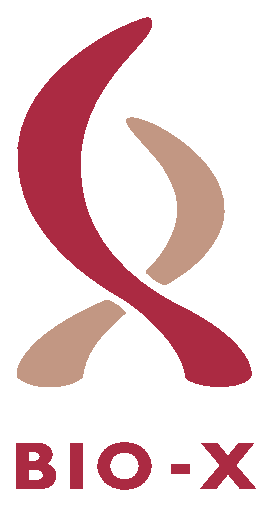
\includegraphics[height=5cm]{bio-x.eps}%
    \hspace{0.5cm}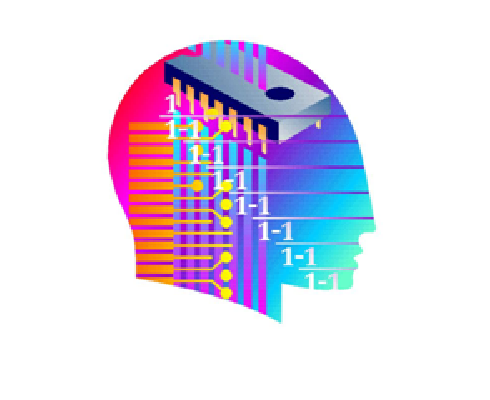
\includegraphics[height=5cm]{swartz.eps}}

%%%%%%%%%%%%%%%%%%%%%%%%%%%%%%%%%%%%%%%%%%%%%%%%%%%%%%%%%%%%%%%%%%%%%%%%%%%

%---------Setup--------------------------------------------------------

\begin{document}

\begin{frame}{}

\begin{columns}[t]

%%%%%%%%%%%%%%%%%%%%%%%%%%%%%%%%%%%%%%%%%%%%%%%%%%%%%%%%%%%%%%%%%%%%%%%%%%%
%-------------Beginning--------------------------------------------------------

%-------------Column--------------------------------------------------------
\begin{column}{0.26\linewidth}

\section{Background}

%-------------Box--------------------------------------------------------

\begin{block}{Storage capacity of synaptic memory}
%
% \begin{itemize}
%   \item Capacity limited by new memories overwriting old
%   \item Hopfield capacity $\propto N$ requires unbounded synaptic strengths.
%   \item Bounded synapses $\implies$ capacity $\propto\log N$.
%   \item Trade-off between learning \& remembering.
%   \item Can be ameliorated by using metaplasticity in complex synapses
% \end{itemize}
%
 A classical perceptron, when used as a recognition memory device, has a memory capacity proportional to the number of synapses, $N$.

 \vp However, this requires synapses to have a dynamic range also $\propto N$.
 
 \vp If synaptic efficacies are limited to a fixed dynamic range, this introduces a strong tradeoff between learning and forgetting due to new memories overwriting old.
 If we wish to store new memories rapidly, then memory capacity is $\CO(\log N)$.
 \\ \citerr{amit1992constraints,amit1994learning}

 \vp To circumvent this tradeoff, it is essential to enlarge our theoretical conception of a synapse as a single number.
 %
\end{block}

%-------------Box--------------------------------------------------------

\begin{block}{Complex synapses}
%
 \begin{minipage}[t]{0.47\linewidth}
   In reality, a synapse is a complex dynamical system.

   \vp We will describe a synapse by stochastic processes on a finite number of states, $M$.

   \vp Potentiation and depression cause transitions between these states.

   \vp
   \begin{center}
     \aligntop{\includegraphics[width=0.76\linewidth]{synapse.svg}}
   \end{center}
 \end{minipage}
 %
 %\hspace{1cm}
 %
 \begin{minipage}[t]{0.49\linewidth}
   \begin{center}
    \aligntop{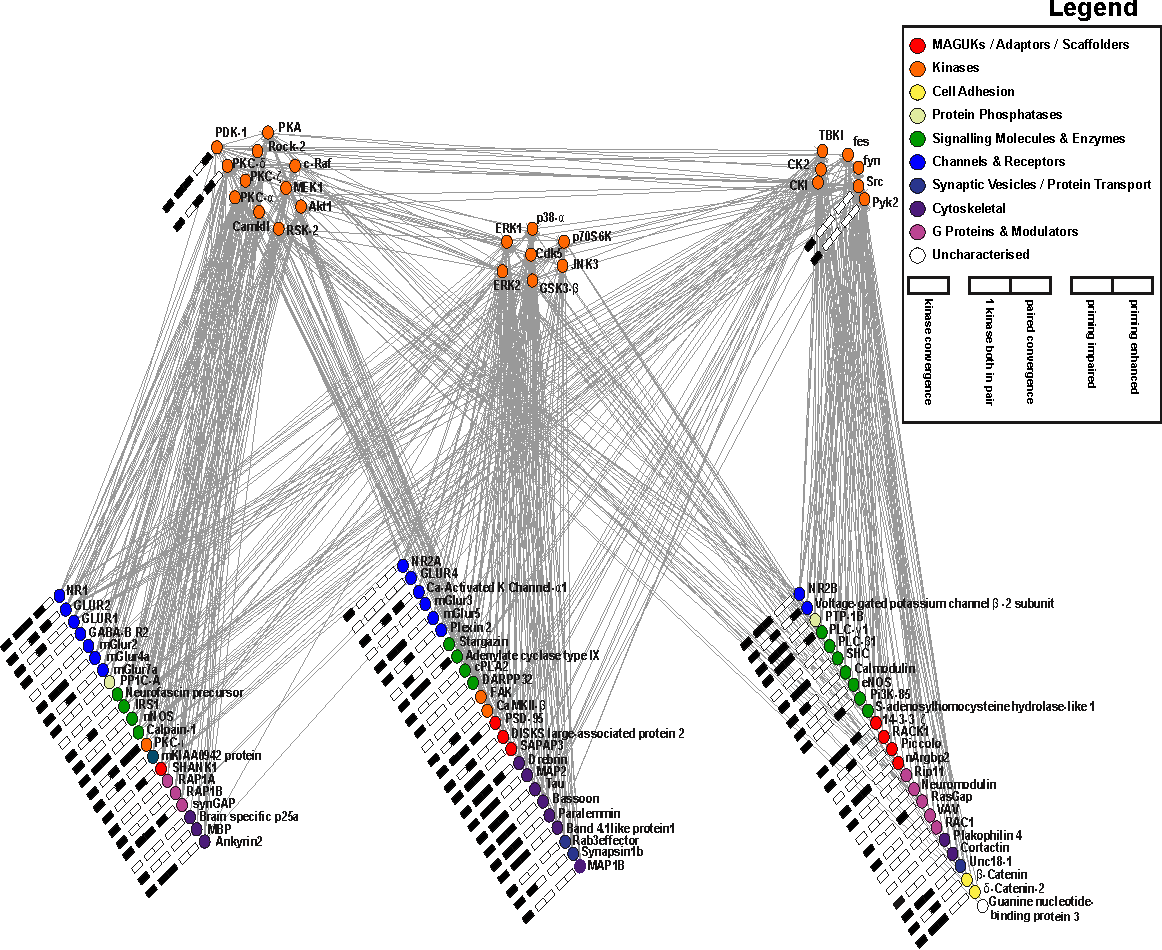
\includegraphics[width=0.96\linewidth]{2000102CobaFig4.pdf}}
   \end{center}
    \citerr{Coba2009phosphorylation}

   \begin{center}
   \aligntop{\includegraphics[width=0.32\linewidth]{pot.svg}}
   \hspace{2cm}
   \aligntop{\includegraphics[width=0.32\linewidth]{dep.svg}}
   \end{center}
 \end{minipage}
%
\end{block}

%-------------Box--------------------------------------------------------

\begin{block}{Cascade and serial models}
%
 Two example models of complex synapses.
 \begin{center}
% \parbox[t]{30cm}{
  \aligntop{\includegraphics[width=0.35\linewidth]{cascade.svg}}
  \hspace{2cm}
  \aligntop{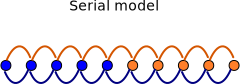
\includegraphics[width=0.35\linewidth]{serial.svg}}
% }
 \end{center}
 \citerr{Fusi2005cascade,Leibold2008serial}

 These have different memory storage properties
 \begin{center}
 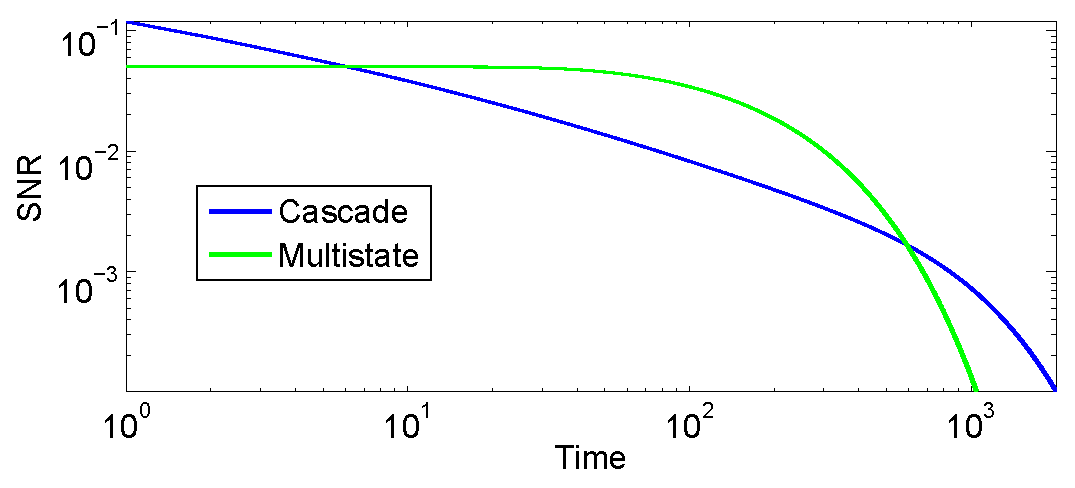
\includegraphics[width=0.5\linewidth]{cascms.eps}
 \end{center}
%
\end{block}


%-------------Box--------------------------------------------------------

\begin{block}{Questions}
%
 \begin{itemize}
   \item Can we understand the space of \emph{all possible} synaptic models?
   \item How does the structure (topology) of a synaptic model affect its function (memory curve)?
   \item How does synaptic complexity (number of states) extend the frontiers of possibility for memory?
   \item Which synaptic state transition topologies maximize measures of memory?
 \end{itemize}
%
\end{block}


%-------------Column--------------------------------------------------------
\end{column}

%-------------Column--------------------------------------------------------
\begin{column}{0.415\linewidth}

\section{Framework}

%-------------Box--------------------------------------------------------

\begin{block}{Synaptic state transition models}
%
% We have $N$ synapses with $n$ internal states.
%
 We have two Markov processes describing transition probabilities for potentiation, $\M\pot$, and depression, $\M\dep$.

 \vp Plasticity events are potentiating with probability $f\pot$ and depressing with probability $f\dep$.

 \vp After the memory we are tracking, subsequent plasticity events occur at rate $r$, with transition probabilities
 %
 \begin{equation*}
   \M\frg = f\pot\M\pot + f\dep\M\dep.
 \end{equation*}
 %
 This will eventually return it to the equilibrium distribution, $\eq$.

 \citerr{Fusi2005cascade,Fusi2007multistate,Barrett2008discrete}
%
\end{block}

%-------------Box--------------------------------------------------------

\begin{block}{Memory curve}
%
 We use the ideal observer approach: read synaptic weights directly.
 This is an upper bound on what could be read from network activity.

 The reconstruction probability of a single synapse is:
 %
 \begin{equation*}
   s(t) = f\pot P(\text{strong},t\mid\text{pot},0) + f\dep P(\text{weak},t\mid\text{dep},0)
 \end{equation*}
 %
 Alternatively, if $\W$ is an $N$-element vector of synaptic strengths,
 %
 \begin{equation*}
   \begin{aligned}
     \text{Signal} &= \av{\W_\text{ideal} \cdot \W(t) -  \W_\text{ideal} \cdot \W(\infty)}, \\
     \text{Noise} &= \sqrt{\var\prn{\W_\text{ideal} \cdot \W(\infty)}}.
   \end{aligned}
 \end{equation*}
 %
 If we assume there are no correlations between different synapses, the signal-to-noise ratio is:
 %
 \begin{equation*}
   \SNR(t) \sim \sqrt{N}(s(t)-s(\infty)).
 \end{equation*}
 %
%
\end{block}


\section{Upper bounds on performance}

%-------------Box--------------------------------------------------------

\begin{block}{Area bound}
%
 \parbox[c]{0.6\linewidth}{
 % We can show that the area under the SNR curve is bounded:
 % %
 % \begin{equation*}
 %   A \leq \sqrt{N}(n-1)/r.
 % \end{equation*}
 % %
 % This is saturated by a transition diagram with a linear chain topology.
 %
 % \vp This leads to a bound on the memory lifetime of \emph{any} synaptic model:
 % %
 % \begin{equation*}
 % \begin{aligned}
 %   \SNR(\text{lifetime})&=1
 %   &\qquad
 %   \implies
 %   \quad
 %   \text{lifetime} &< A.
 % \end{aligned}
 % \end{equation*}
 % %
  The memory lifetime is bounded by the area under the SNR curve:
  %
  \begin{equation*}
  \begin{aligned}
    \SNR(\text{lifetime})&=1
    &\qquad
    \implies
    \quad
    \text{lifetime} &< A.
  \end{aligned}
  \end{equation*}
  %
  We can show that this area has an upper bound:
  %
  \begin{equation*}
    A \leq \sqrt{N}(M-1)/r.
  \end{equation*}
  %
  This is saturated by a transition diagram with a linear chain topology.
 }
 \hfill
 \parbox[c]{0.37\linewidth}{
  %
  \begin{center}
    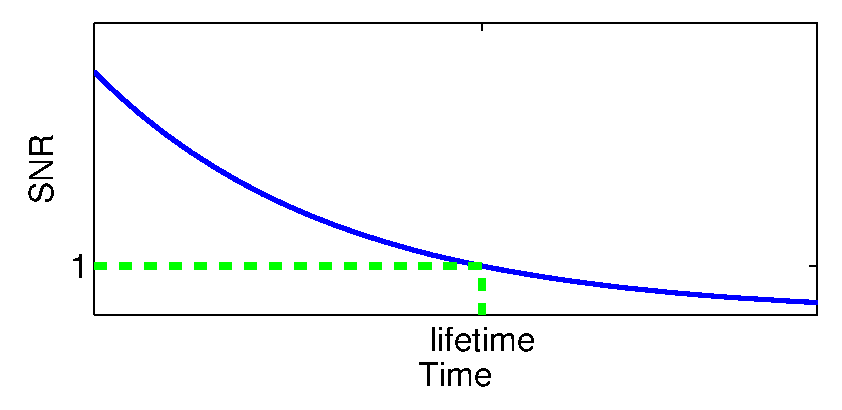
\includegraphics[width=0.9375\linewidth]{lifetime.eps}
  \end{center}
  %
 }
%
\end{block}

%-------------Box--------------------------------------------------------

\begin{block}{Proof: Impose an ordering on the states}
%
 Let $\fpt_{ij}$ be the mean first passage time from state $i$ to state $j$.
 The following quantity
 %
 \begin{equation*}
   \eta = \sum_j \fpt_{ij} \eq_j,
 \end{equation*}
 %
 is independent of the initial state $i$.
 It is known as Kemeney's constant. \citerr{kemeny1960finite}

 \vp We define:
 %
 \begin{equation*}
   \eta^+_i = \sum_{j\in\text{strong}} \fpt_{ij} \eq_j,
   \qquad
   \eta^-_i = \sum_{j\in\text{weak}} \fpt_{ij} \eq_j.
 \end{equation*}
 %
 These measure ``distance'' to the strong/weak states.
 They can be used to arrange the states in an order (increasing $\eta^-$ or decreasing $\eta^+$).
%
\end{block}

%-------------Box--------------------------------------------------------

\begin{block}{Maximal area}
%
 Given any synaptic model, we can construct one with a linear chain topology that has
 \parbox[c]{0.34\linewidth}{
  \begin{itemize}
    \item the same state order,
    \item the same equilibrium distribution,
    \item a larger area.
  \end{itemize}
 }
 \parbox[c]{0.34\linewidth}{
  %
  \begin{center}
    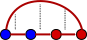
\includegraphics[width=0.4\linewidth]{shortcut.svg}
  \end{center}
  %
 }

 Uses a deformation that reduces ``shortcut'' transition probabilities and increases the bypassed ``direct'' ones.

 \vp The area of this model is
 %
 \begin{equation*}
   A = \frac{2\sqrt{N}}{r}\sum_k \eq_k \abs{k-\av{k}}.
 \end{equation*}
 %
 This is maximized when the equilibrium probability distribution is concentrated at both ends.
%
\end{block}





%-------------Column--------------------------------------------------------
\end{column}

%-------------Column--------------------------------------------------------
\begin{column}{0.3\linewidth}


%-------------Box--------------------------------------------------------

\begin{block}{Initial SNR bound}
%
 Initial SNR is closely related to equilibrium flux between strong \& weak states
 %
 \begin{equation*}
   \SNR(0) \leq \frac{4\sqrt{N}}{r}\,\F_{-+}.
 \end{equation*}
 %

 \vp
 Maximized when %\parbox[t]{0.7\linewidth}{
 potentiation guarantees $\W\to$ strong, %\\
 depression guarantees $\W\to$ weak.
 %                                                                                                                  }
% %
% \begin{center}
%   \includegraphics[height=3cm]{max_init_pot.svg}
%   \hspace{2cm}
%   \includegraphics[height=3cm]{max_init_dep.svg}
% \end{center}
%
% \vp \lto\ Equivalent to two-state model
%  \begin{center}
%  Transitions:
%   \parbox{2cm}{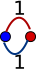
\includegraphics[height=4cm]{binary_det.svg}}
%   $\implies\snr(t)=\sqrt{N}\,(4 f\pot f\dep)\,\e^{-rt}.$
%  \end{center}
 \begin{center}
   \alignmid{\includegraphics[height=0.08\linewidth]{max_init_pot.svg}}
   \hspace{0.5cm}
   \alignmid{\includegraphics[height=0.08\linewidth]{max_init_dep.svg}}
   \hspace{1cm}
  \lto\ Equivalent to:
   \hspace{0.5cm}
   \alignmid{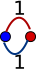
\includegraphics[height=0.1\linewidth]{binary_det.svg}}
   $\implies\snr(t)=\sqrt{N}\,(4 f\pot f\dep)\,\e^{-rt}.$
  \end{center}

 \vp Maximal initial SNR:\hspace{2cm}
 %
 $
   \snr(0) \leq \sqrt{N}.
 $
%
\end{block}


\section{The memory envelope}


%-------------Box--------------------------------------------------------

\begin{block}{The frontiers of possibility: a maximal SNR curve}
%
 Markovian learning and forgetting $\implies$ SNR is a sum of decaying exponentials.

 \vp Optimizing the SNR \emph{at one time}, $t_0$, over the space of such curves,
 subject to upper bounds on initial SNR and area,
 yields an upper bound on SNR at $t_0$ for \emph{any} synaptic model.
 The resulting optimal memory curve is a single exponential
 (optimizing at two or more well separated times requires multiple exponentials).

 \vp Varying $t_0$ yields a memory envelope curve with a power law tail.

\vp
\parbox[c]{0.45\linewidth}{
 \begin{center}
   \aligntop{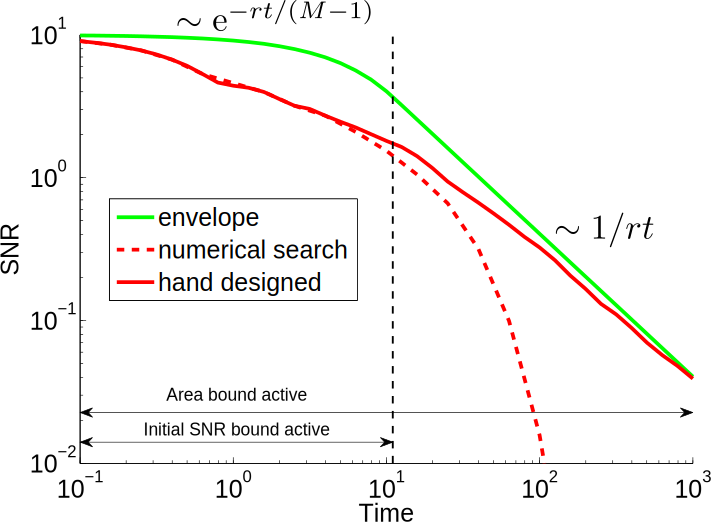
\includegraphics[width=0.89\linewidth]{env.svg}}
 \end{center}
}
\hspace{0.5cm}
\parbox[c]{0.45\linewidth}{
 %
   Early times: (varying $M$)
   %
   \begin{center}
  %   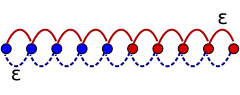
\includegraphics[width=6cm]{multistate_shorten.svg}
     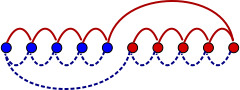
\includegraphics[width=0.7\linewidth]{diffjump.svg}
   \end{center}
   %
  % \note[item]{shorten length of chain, keeping deterministic}

   %
   \vp Late times: (varying $\varepsilon$)
   %
   \begin{center}
     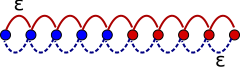
\includegraphics[width=0.7\linewidth]{multistate_sticky.svg}
   \end{center}
   %
%% Proven:
% \begin{equation*}
%  \begin{aligned}
%   \text{Proven envelope} &\sim \sqrt{N}
%     \begin{cases}
%       \CO(1)                  & rt_0 <\CO(n),\\
%       \CO\prn{\frac{n}{rt_0}} & rt_0 >\CO(n).
%     \end{cases}
%   \\
%%  \end{aligned}
%% \end{equation*}
%% %
%% Conjectured:
%% %
%% \begin{equation*}
%%  \begin{aligned}
%   \text{Conj.\ envelope} &\sim \sqrt{N}
%     \begin{cases}
%       \CO\prn{\frac{1}{\sqrt{rt_0}}}  & rt_0 <\CO(n^2),\\
%       \CO\prn{\frac{n}{rt_0}}         & rt_0 >\CO(n^2).
%     \end{cases}
%  \end{aligned}
% \end{equation*}
 %
}
%
\end{block}
%
%%-------------Box--------------------------------------------------------
%
%\begin{block}{Extra constraint: limits of diffusive learning and forgetting}
%%
% The envelope above may not be tight.
% We conjecture an additional constraint, which would yield a tight envelope (dashed line above).
% Schematically, mode by mode:
% %
% \begin{equation*}
%   \SNR(0)\sqrt{\text{time-scale}} \leq \sqrt{N}\cdot \CO(1).
% \end{equation*}
% %
% We have found no model that can exceed this bound.
% It is saturated by a diffusive chain:
% %
% \begin{equation*}
%   \SNR(0) \sim \frac{1}{n},
%   \qquad
%   \text{time-scale} \sim n^2.
% \end{equation*}
% %
%%
%\end{block}
%
%%-------------Box--------------------------------------------------------
%
%\begin{block}{Maximum lifetime}
%%
% We can use the envelope to get a stricter bound on the lifetime of a memory
% %
% \begin{equation*}
% \begin{aligned}
%   \operatorname{Envelope}(\text{max lifetime}) = 1, \qquad
%   \text{max lifetime}  = \frac{\sqrt{N}(n-1)}{\e r}.
% \end{aligned}
% \end{equation*}
% %
%%
%\end{block}

%\section{}

%-------------Box--------------------------------------------------------

\begin{block}{Summary}
%
  \begin{itemize}
    \item We have formulated a general theory of learning and memory with complex synapses.
    \item We can impose an order on the internal states of a synapse through the theory of first passage times.
    \item The area under the memory curve of any synaptic transition diagram cannot exceed that of a linear chain with the same equilibrium probability distribution.
    \item We find a memory envelope: a single curve that cannot be exceeded by the memory curve of \emph{any} synaptic model.
    \item    Synaptic complexity ($M$ internal states) raises the memory envelope linearly in $n$ for times $> \CO(M)$.
%    \item For times $< \CO(n^2)$ we conjecture the close to optimal synaptic model that reaches the envelope exploits deterministic transitions, resulting in diffusive forgetting.
  \end{itemize}
%
\end{block}

%-------------Box--------------------------------------------------------

\begin{block}{References}
%
 {\tiny
 \bibliographystyle{unsrt_poster}
 \bibliography{neuro,maths}
 }
%
\end{block}

%-------------Box--------------------------------------------------------

\begin{block}{Acknowledgements}
%
 SL and SG thank the Swartz Foundation, Burroughs Wellcome Foundation, Stanford Bio-X Neuroventures, Genentech and DARPA for funding, and Larry Abbott, Stefano Fusi, Marcus Benna, David Sussillo and Jascha Sohl-Dickstein for useful conversations.

%
\end{block}


\end{column}




%%%%%%%%%%%%%%%%%%%%%%%%%%%%%%%%%%%%%%%%%%%%%%%%%%%%%%%%%%%%%%%%%%%%%%%%%%%
%-----End----------------------------------------------------------------

\end{columns}

\end{frame}

\end{document}
